\documentclass[12pt,a4paper,onecolumn,oneside]{book}
%\usepackage{draftcopy}
\reversemarginpar
\newcommand{\meek}{\marginpar[\hfill\fbox{!}]{\fbox{!}}}
\parskip 1.5ex
%\parindent 1.5em
%\thispagestyle{empty}
%\pagestyle{plain}
%\pagenumbering{arabic}
%\setlength{\topmargin}{0pt}
%\setlength{\headheight}{0pt}
%\setlength{\headsep}{0pt}
%\setlength{\topskip}{0pt}
\setlength{\textheight}{220mm}
%\setlength{\footskip}{5ex}
\setlength{\oddsidemargin}{0pt}
\setlength{\evensidemargin}{0pt}
\setlength{\textwidth}{160mm}
\usepackage[dvips]{graphics,color}
\usepackage{helvet}
\renewcommand{\familydefault}{\sfdefault}
\newcounter{ch-variables}
\newcounter{ch-variables-page}
\newcounter{teaMakePage}
\newcounter{seedVariable}
\makeindex
\begin{document}
\begin{sffamily}

\definecolor{rtb-black}{rgb}  {0.0, 0.0, 0.0}
\definecolor{rtb-navy}{rgb}   {0.0, 0.0, 0.5}
\definecolor{rtb-green}{rgb}  {0.0, 0.5, 0.0}
\definecolor{rtb-teal}{rgb}   {0.0, 0.5, 0.5}
\definecolor{rtb-maroon}{rgb} {0.5, 0.0, 0.0}
\definecolor{rtb-purple}{rgb} {0.5, 0.0, 0.5}
\definecolor{rtb-olive}{rgb}  {0.5, 0.5, 0.0}
\definecolor{rtb-silver}{rgb} {0.7, 0.7, 0.7}
\definecolor{rtb-grey}{rgb}   {0.5, 0.5, 0.5}
\definecolor{rtb-blue}{rgb}   {0.0, 0.0, 1.0}
\definecolor{rtb-lime}{rgb}   {0.0, 1.0, 0.0}
\definecolor{rtb-aqua}{rgb}   {0.0, 1.0, 1.0}
\definecolor{rtb-red}{rgb}    {1.0, 0.0, 0.0}
\definecolor{rtb-fuchsia}{rgb}{1.0, 0.0, 1.0}
\definecolor{rtb-yellow}{rgb} {1.0, 1.0, 0.0}
\definecolor{rtb-white}{rgb}  {1.0, 1.0, 1.0}

\begin{titlepage}
\title{Return to Basic\\Reference Manual}
\author{Gordon Henderson\\gordon@drogon.net\\
\copyright 2012}
%\date{January 2012}
\maketitle
\end{titlepage}

\frontmatter
\pagestyle{plain}
\addcontentsline{toc}{chapter}{Preface}
\section*{Preface}
\index{Preface}

\vspace{3ex}
\noindent
Return to Basic (RTB) is a project to re-create a modern version of
the BASIC interpreter and programming environment popular in the
late 1970s through the 1980s on the popular 8-bit microprocessor
systems such as the Apple ][ series, BBC Micro and Commodore PET
as well as the various Sinclair systems and a whole host of others
too numerous to mention. The intention is to present an easy to use
environment for young (and old) people to learn to write computer
programs using an interactive system that's quick and easy to use.
\index{Apple}\index{BBC}\index{Sinclair}\index{Commodore PET}

BASIC (Beginners All-purpose Symbolic Instruction Code) is regarded as
somewhat old-fashioned in todays world (c2012), but I believe it still
has a place in the teaching and learning of computer programming. It
arguably has many faults and has been criticised for encouraging bad
programming practices, however RTB is a new implementation, capable
of using modern structured programing techniques including named
functions and procedures (which support recursion, if desired) and
structured looping constructs. Also, while this manual demonstrates the
use of the GOTO instruction it does discourage it and quickly moves on
to demonstrating newer techniques. You can even write RTB programs without
line numbers and merge library files of procedures and functions together.

RTB is not intended to be used as a serious programming system --
While it has the capabilities to write a large financial package in, I
do not expect people to write the many, varied and large packages that
were commonly written in BASIC in those early days, but rather to be
used as a way to introduce programming in an easy to understand manner.

RTB features several graphical systems that were popular in those early
microprocessor years -- both a low and high resolution colour graphics
system as well as ``turtle'' graphics with simplified colour and angle
handling. It is more than capable of being used to write simple games
and animations in.

I would like to think that pre-teen children can be introduced to
programming using RTB -- the only prerequisite is a desire to learn and
the ability to type some simple instructions into a computer. It doesn't
even need a mouse!

This manual is intended to be used as a reference manual for RTB. It
lists all the major programming constructs with a small number of examples.
\vfill
{\hfill\em Gordon Henderson, February 2012}
\newpage
\addcontentsline{toc}{chapter}{Trademarks and Acknowledgements}
\index{Trademarks}\index{Acknowledgements}
\section*{Trademarks and Acknowledgements}
Raspberry Pi is a registered trademark of the Raspberry Pi Foundation


\addcontentsline{toc}{chapter}{Warranty and Copying}
\index{Warranty}\index{Copying}
\section*{Warranty and Copying}
\begin{verbatim}
 * This document is part of RTB:
 *	Return To Basic
 *	http://projects.drogon.net/return-to-basic
 *
 *    RTB is free software: you can redistribute it and/or modify
 *    it under the terms of the GNU General Public License as published by
 *    the Free Software Foundation, either version 3 of the License, or
 *    (at your option) any later version.
 *
 *    RTB is distributed in the hope that it will be useful,
 *    but WITHOUT ANY WARRANTY; without even the implied warranty of
 *    MERCHANTABILITY or FITNESS FOR A PARTICULAR PURPOSE.  See the
 *    GNU General Public License for more details.
 *
 *    You should have received a copy of the GNU General Public License
 *    along with RTB.  If not, see <http://www.gnu.org/licenses/>.
\end{verbatim}


\tableofcontents
\mainmatter
\pagestyle{headings}
\chapter{Introduction}
\section{Audience}
\index{Audience}
This manual is aimed at people who may already have a familiarity with
BASIC or other high-level languages. It's mainly a reference manual
for the language, but that are a few examples and tutorials.

The manual will assume that you understand most common principles
of computing and know concepts like volatile and non-volatile storage
and so on and how to type some commands into your computer.

And although it's a reference manual, there are one or two little
examples and tutorials along the way for you to try out.

\section{Conventions Used in this Manual}
\index{Conventions}
Keeping things simple is the aim here, so there are only really 3
things to look out for\footnote{OK, Possibly four as there may be
the occasional footnote at the bottom of a page, so look out for them
too.}. The first is that anything you may need to type into a computer
running RTB, or anything it prints will be in this {\tt typewriter}
style font. The second is that anything of some importance, such as a
name of an algorithm is emphasised {\em like this}.

The \meek final thing to look out for is a warning, or just something
that may be important to remember. It's represented by a warning
exclamation point in a box to the side of the text. As demonstrated in
this paragraph.\newpage
\index{Warning}

If you know what you're doing, here are some brief differences between
RTB and a ``classic'' BASIC:
\begin{itemize}
\item RTB does not allow multiple statements on one line.
One statement per line only.
\item Variable names can be of almost any length and upper/lower case
is significant.
\item {\tt IF} statements must have {\tt THEN} (So no {\tt IF\dots\
num = 4}, or {\tt IF\dots\ GOTO 10}, it must be the full {\tt IF\dots\
THEN GOTO 10}, or {\tt IF\dots\ THEN a = 7}, etc.)
\item In {\tt FOR} loops, there is no {\tt NEXT} instruction -- it's
replaced by the {\tt CYCLE\dots REPEAT} construct.
\item Named procedures and functions. (Which can be called recursively)
\item Local variables inside user-defined procedures and functions.
\item A single looping construct ({\tt CYCLE\dots REPEAT}) which can be
modified with {\tt FOR}, {\tt WHILE} and {\tt UNTIL} constructs.
\item {\tt BREAK} and {\tt CONTINUE} as part of the looping construct.
\item Arrays start at zero and go up to and include the number in the
{\tt DIM} statement. ie. the {\tt DIM} statement specifies the size of
the array plus one.
\end{itemize}
Additionally (where supported) the graphical systems may well be new or
different to you. RTB incorporates simple block/line graphics as well
as turtle graphics using a variety of angle modes (degrees, radians
and clock).

\chapter{The RTB environment}

RTB is primarily designed to run on computers running Linux. In the
fullness of time, both MS windows and Apple Mac versions may be made
available, but for now it's Linux only.

On the Raspberry Pi, there are some additional features to make use of
the Pi's GPIO facility.
\index{PC}\index{Apple}\index{Mac}\index{Raspberry Pi}\index{Linux}

Starting RTB may vary from one Linux system another, however opening up
a text (or command/shell) terminal and typing

{\tt rtb}

at the prompt will usually get things going for you.

Whatever the system, once RTB has started it should look the same. There
will be a keyboard to type commands into, this is connected to the main
computer which should be connected to a screen or display of some sort. A
Raspberry Pi may even be connected to your home TV set.

When it's setup and ready, the screen should be clear apart from some
introductory text and a prompt. It will probably look something like this:
\begin{verbatim}
  Return to Basic version 1.0 
  Ready
  >
\end{verbatim}
The ``$>$'' symbol is the prompt. It's presence means that RTB is ready to
accept commands and program lines typed into it.
\index{Prompt}

\section{A quick introduction to BASIC}
(You may wish to skip this if you are familiar with BASIC)

BASIC and therefore RTB has three basic modes of operation: Immediate
mode, program store mode and program run mode.
\index{Modes}

\section{Immediate mode}
\index{Immediate mode}
This is when commands you type into the system are executed immediately.
You can use this mode to perform simple calculations, examine the state
of variables and do other ``housekeeping'' tasks such as saving and loading
your programs, and so on.

\noindent
A few examples:
\begin{verbatim}
  PRINT "Hello"
  PRINT "My name is: Gordon Henderson"
\end{verbatim}
Calculator:
\begin{verbatim}
  PRINT 1+2
  PRINT 1+2*3
\end{verbatim}
\index{Calculator}

A \meek quick note about the calculator and symbols used. There isn't a
proper divide symbol on your keyboard: $\div$ so we use the forward-slash
character instead: {\tt /} and similarly rather than use the multiply
character: $\times$ we use the asterisk: {\tt *}.

\section{Run mode}\index{Run mode}
This is simply when a program is running. To start a stored program,
use the {\tt RUN} command. The program will stop running when it
encounters a {\tt STOP} or {\tt END} instruction, or when an error is
detected. You can stop a running program at any time by using the {\tt
ESC}\footnote{Short for {\em Escape}} key at any time.

\section{Stored program mode}
\index{Stored program mode}

This mode allows us to store a program in the computers memory which we
can then execute over and over again. We differentiate immediate mode
from stored program mode by giving each line we type a line number at
the start of the line.

\noindent
To enter a simple program:
\begin{verbatim}
  10 PRINT 1 + 2 * 3
  20 END
\end{verbatim}
Remember to press the {\tt ENTER} key after every line.

To insert a line of code between two existing lines, you can use a
line-number in-between the existing numbers, so using the example above,
to insert a line we can type:
\begin{verbatim}
   5 PRINT "The answer to 1 + 2 * 3 is:"
\end{verbatim}
Verify it with the {\tt LIST} command -- and note that the computer has
added line 5 before line 10, which is what you expect because computers
are boringly good at counting. Run the program again and note the output.

\noindent
Add this line:
\begin{verbatim}
  15 PRINT "Six times seven is: "; 6 * 7
\end{verbatim}
list and run the program again. 

A few final notes here: If you enter a new line with the same number as
one already entered, it will delete the one stored and replace it with
the one you entered, or if you enter a line number and nothing else
(just press {\tt ENTER} after the line number, then it will delete any
line with that number.

It \meek is also good practice to regularly save your work.  Imagine the
frustrations of having a power cut which will lose all your work
so-far\dots

\section{BASIC}
\index{BASIC}
This is the essence of BASIC programming. You can enter commands to
be executed immediately, or enter program lines (with line numbers)
which the computer will store for as long as it's turned on, or until
you delete them by overwriting them, or using the {\tt NEW} command.

List your programs with the {\tt LIST} command and run them with the
{\tt RUN} command.

When entering new programs it is suggested to start at line number 10
and go up in 10s. That way, there is plenty of room to enter new lines
in-between if required. (But there's always the {\tt RENUMBER}
\index{RENUMBER} command if you run out of space)\\

\chapter{The command-line}\index{Command line}
The command line is the general term for typing commands and 
program lines into the system, however it has a few features to
make your life easier.

\section{Editing}\index{Command line!Editing}
As you type characters into the system, you may make mistakes. To correct
them you can use several differenet keys. The important one is probably
the {\tt Backspace} key. Usually a big key to the top-right of the main
keyboard with an arrow pointing to the left. This will erase characters
you've typed and move the cursor to the left, however there are more
efficient ways to deal with the like you're typing noted below.

Some of  the command characters lsited below you access with the {\tt
Control} key. This is labelled as {\tt Ctrl} on most keyboards and
works like the {\tt Shift} keys in that you push it, keep it pushed,
then type another character before releasing them both.

\begin{description}
\item[{\tt Ctrl-A}, {\tt Ctrl-E}:] Move the cursor to the start or the
end of the line respectively. You can also use the {\tt Home} and {\tt End}
keys if your keyboard has them.
\item[{\tt $\leftarrow$ (Left)} and {\tt $\rightarrow$ (Right)}:] arrow
keys (not to be confused with the {\tt Backspace} key) move the cursor
one character to the left or right of the typed line.
\item[{\tt Ctrl-D}:] Delete the character under the cursor. You can also
use the {\tt Del} or {\tt Delete} key if your keyboard has one.
\item[{\tt Backspace}:] Deletes the character to the Left of the cursor)
\item[{\tt Ctrl-S}:] Swap the character under the cursor with the character
immediately to the right. Handy for those who type the as teh like me\dots
\item[{\tt Ctrl-F}:] Find the next occurance of the next character typed.
E.g. {\tt Ctrl-F} followed by {\tt G} will make the cursor jump to
the next {\tt G} in the line. {\tt Ctrl-F} followed by another {\tt
Ctrl-F} will repeat the last find. 
\item[{\tt Esc}:] Abandon entering this entire line.
\end{description}

\section{History}
\index{Command line!History}
The RTB command line remembers the past 50 lines that you type in,
and you can use the $\uparrow$ ({\tt Up}) and $\downarrow$ ({\tt Down})
arrow keys on your keyboard to scroll through past things you've typed
in. This will enable you to quickly fix a mistake in a line already
in the system, or a line you typed in which remoted an error after you
pressed the {\em Enter} key.

\section{Editing program lines}
\index{Command line!Edit program lines}
If you spot a mistake in a program line and you can't find it in the
history, then you can enter the {\tt ED} command followed by the line
number. E.g. {\tt ED 10} will then present line 10 as if you had
re-typed it, but not yet pressed {\em Enter} so you can change the line
as required.

\chapter{Immediate mode commands}\index{Immediate mode commands}

In immediate mode, as well as executing simple print instructions as
well as other instructions you can use within a program, there are several
commands which can only be executed in immediate mode.

\begin{description}
\item[{\tt LIST [[first] last]}:]\index{LIST}
This lists the program stored in memory to the screen. You can pause the
listing with the space-bar and terminate it with the escape key. If {\tt
first} is given, then only that line will be listed. If both {\tt first}
and {\tt last} are given, then lines in that range will be listed.
\item[{\tt SAVE [filename]}:]\index{SAVE}
Saves your program to the local non-volatile storage. {\tt filename} is
the name of the file you wish to save and may not contain spaces. If you
have already saved a file, then you can subsequently execute {\tt SAVE}
without the filename and it will overwrite the last file saved. (This is
``safe'' as it's reset when you load a new program or use the {\tt NEW}
command)
\item[{\tt SAVENN [filename]}:]\index{SAVENN}
Same as the normal {\tt SAVE} command, but saves with No line
Numbers. You can only save without line numbers if your program has no
{\tt GOTO} or {\tt GOSUB} statements and no {\tt RESTORE} statements
with a line-number.
\item[{\tt LOAD filename}:]\index{LOAD}
Loads in a program from the local non-volatile storage. As with {\tt
SAVE}, you need to supply the filename without any quotes.
\item[{\tt DIR [directory]}:]\index{DIR}
Lists the RTB files in your current working directory, or the given
directory (without quotes)
\item[{\tt NEW}:]\index{NEW}
Deletes the program in memory. There is no verification and once it's
gone, it's gone. Remember to save first!
\item[{\tt RUN}:]\index{RUN}
Runs the program in memory. You may give a line number and the
program will start from that number rather than the first line in the
program. Note that using {\tt RUN} will clear all variables.
\item[{\tt CONT}:]\index{CONT}
Continues program execution after a {\tt STOP}\index{STOP}
instruction. Variables are not cleared.
\item[{\tt CLEAR}:]\index{CLEAR}
Clears all variables and deletes all arrays. It also removes any active
sprites from the screen.  Stopped programs may not be continued after
a {\tt CLEAR} command.
\item[{\tt TRON}:]\index{TRON}
Turns line-number tracing on. As each line is executed, it's number is
printed to the text console that RTB was started from.
\item[{\tt TROFF}:]\index{TROFF}
Turns line number tracing off.
\item[{\tt ED linenumber}:]\index{ED}
Edit the line given.
\item[{\tt RENUMBER [start [inc [first [last]]]]}:]\index{RENUMBER}
This renumbers your program - by default it will start at 100 and go
in increments of 10, however you can change this as follows: The {\tt
start} and {\tt inc} parameters specify the new starting line number and
increment, the {\tt first} and {\tt last} parameters specify the first
and last {\em exiting} line numbers to renumber. Using this latter way,
you can move lines in the program, but beware of overlaps.

If an overlap does occur, then renumbering will stop at that point and
you may find your program to be somewhat scrambled\dots Please make sure
you save your program before renumbering!

\item[{\tt VERSION}:]\index{VERSION}
Print the current version of RTB.
\item[{\tt EXIT}:]\index{EXIT}
Exit RTB and return to the environment you started RTB in.
\end{description}

\section{File names}
\index{File names}
The system you run RTB on may have its own rules
about what a filename can look like, and whether the name is
case-sensitive. (ie. UPPER/lower case letters -- are they considered the
same, or different?) In the Linux environment then case is significant. If
you're not sure, just stick to simple names without spaces. If you're
subsequently looking at the files outside the RTB environment note that
the filenames will have the characters {\tt .rtb} appended to it.

\chapter{Comments}
\index{Comments}

It's always a good idea to include comments in your programs, and RTB
provides 2 methods to help you do this.

Firstly, there is the traditional {\tt REM} statement. Short for
``Remark''.  Secondly there is the {\tt //} statement which is
common in many other programming languages.

{\tt REM} must appear at the start of a program line, but {\ //} may
appear anywhere in a line - and anything after the {\tt //} is ignored.

Examples:
\begin{verbatim}
  100 REM This is a demonstration of comments
  110 //
  120 REM // on its own can be used to separate program sections.
  130 //
  140 // The line below is allowed:
  150 LET test = 42 // Set test to 42
  160 //
  170 // But the line below this is not allowed:
  180 LET test = 42 REM Set test to 42
\end{verbatim}

\chapter{Flow Control}
\index{Flow Control}
Programs are normally executed in line-number order, one after the other.
There are many ways in which we can alter the flow of our programs, but
the traditional BASIC ones are the {\tt GOTO} and {\tt GOSUB}
instructions.

{\tt GOTO}\index{GOTO} as its name implys causes program execution to go to the line
number listed after the {\tt GOTO} instruction.
\begin{verbatim}
  120 GOTO 315
\end{verbatim}

{\tt GOSUB}\index{GOSUB}\footnote{Go to Subroutine} allows a program to
temporarily jump to a new point and then, upon execution of the {\tt
RETURN} statement, flow resumes at the statement after the {\tt GOSUB}
instruction.

{\tt GOSUB} is designed to be used to allow a piece of code to be executed
over again from different parts of the main program.

Subroutines can call other subroutines and the number of subroutines that
can be called is limited only by the memory capacity of the computer -
some of which is required to keep track of where to return to.

Here is an example -- It's code to print my name:
\begin{verbatim}
  500 REM Simple subroutine to print my name
  510 PRINT "Gordon Henderson"
  580 RETURN
\end{verbatim}
Then, anywhere we need to print my name:
\begin{verbatim}
  100 PRINT "Hello ";
  110 GOSUB 500
  120 PRINT "Good to meet you ";
  130 GOSUB 500
  140 GOTO 100
\end{verbatim}

Subroutines are a good was of saving and re-using code however there
are more modern ways of doing this that removes the need to keep track
of line-numbers.

\section{GOTO and GOSUB -- The great controversy}
\index{GOTO!Controversy}
\index{GOSUB!Controversy}
The use of {\tt GOTO} and {\tt GOSUB} is highly debated and both {\tt
GOTO} and {\tt GOSUB} should be considered deprecated in their use. It
is possible to write fully functional RTB programs without using either
these instructions.

The original version of BASIC did not provide any more means to
control the flow of your code, however newer programming languages have
evolved which do help here, and in some areas the use of the {\tt GOTO}
instruction has been eliminated entirely!

However don't fix the idea in your head that all GOTOs are bad, we
need to balance things up and note that not everyone thinks that GOTOs
are bad -- myself included. Very occasionally, a GOTO can get you out
of a situation in a more elegant manner than some of the constructs
you'll read about next, so don't be afraid of the GOTO, but instead
respect\index{GOTO!Respect} it, try not to use it, but if you have to
use it, then use it well!

\chapter{Variables}
\setcounter{ch-variables}{\value{chapter}}
\setcounter{ch-variables-page}{\value{page}}
\index{Variables}\index{Numbers}\index{Strings}

A variable is an area of computer memory that we can use to store data
in. It has a name associated with it as well as the memory locations
needed to store the data.

\section{Names}
\index{Variables!Names}
Variable names must start with a letter but may otherwise contain any
number of letters and digits and underscores. An example of a variable
name might be: {\tt counter}, or {\tt height} or {\tt numberOfCows}
and so on.

\section{Types}
\index{Variables!Types}
RTB Supports two types of variables; Numbers and Strings. These can
be scalars or arrays.

String variables are differentiated from numeric variables
by having the dollar character appended to them. E.g. {\tt name\$}
or {\tt homeTown\$} and so on.

A number is any decimal value like {\tt 1}, {\tt 3.14}, {\tt
-5}, and so on. Numbers may also be expressed in  scientific
notation. \index{Scientific Notation} and we use the letter ``e''
to represent the power of 10 so {\tt 1.234e7} is {\tt $1.234\times 10^7$},
or {\tt 12340000}. The number range is typically $\pm 10^{308}$.

A string is a sequence of characters, e.g. {\tt "Hello"}, {\tt
"Gordon"} and so on. Strings are always enclosed in double-quotes. The
maximum length of a string is limited by available memory.

\section{Assignment}
\index{Variables!Assignment}
We assign values to variables using the {\tt LET} instruction. e.g.
\index{LET}
\begin{verbatim}
  LET numberOfCows = 0
\end{verbatim}
and we can modify them as follows:
\begin{verbatim}
  LET numberOfCows = cowsInField + cowsInBarn
\end{verbatim}

The \meek {\tt LET} statement is optional.

\section{Numeric operators and Precedence}
\index{Numeric Operators}\index{Precedence}
There are various arithmetic and logical operators that can be
used with numbers.

In order of precedence, they are:
\begin{center}
\begin{tabular}[t]{|c|c|l|}
\hline
{\bf Precedence}	& {\bf Operator}	& {\bf Description}\\
\hline
\hline
{\bf Highest}	&\texttt{\^}	& Exponent, or ``raise to the power of''\\ 
\hline
		&\texttt{-}	& Unary minus\\
\hline
		&\texttt{NOT}	& Logical NOT\\
\hline
		&\texttt{*}\hspace{3mm} 
		\texttt{/}\hspace{3mm}
		\texttt{MOD} 
		\hspace{3mm}
		\texttt{DIV}	& Multiply, Divide, Modulo, Integer Division\\
\hline
		&\texttt{+}\hspace{3mm}
		\texttt{-}	& Addition, Subtraction\\
\hline
		&\texttt{|}\hspace{3mm}
		\texttt{\&}\hspace{3mm}
		\texttt{XOR}	& Logical OR, AND and XOR\\
\hline
		&\texttt{<}\hspace{3mm}
		\texttt{<=}\hspace{3mm}
		\texttt{>}\hspace{3mm}
		\texttt{>=}	& Conditional tests\\
\hline
		&\texttt{=}\hspace{3mm}
		\texttt{<>}	& Conditional Equals and Not Equals\\
\hline
{\bf Lowest}	&\texttt{AND}\hspace{3mm} 
		\texttt{OR}	& Conditional AND and OR\\
\hline
\end{tabular}
\end{center}

You can always use ()'s to alter the evaluation order, if required,
and in some cases they may help to make the code more readable and
obvious.

\section{String Operators}
There is only one string operator - the plus operator which we can use
to concatenate strings.
\begin{verbatim}
  firstName$ = "Gordon"
  lastName$ = "Henderson"
  fullName$ = firstName$ + " " + $lastName$
  PRINT fullName$
\end{verbatim}

\section{Arrays}
\index{Variables!Arrays}
Arrays must be declared before they are first used and we must know the
size of it before-hand. We declare them with the {\tt DIM}\footnote{Short
for Dimension.}\index{DIM} statement.

Arrays can be either numeric or string.  They can not hold mixed values.

Arrays can have more than one dimension - the limit to the number
of dimensions and overall size is program memory.

Arays are used as follows:
\begin{verbatim}
  10 DIM list (4)
  20 list(0) = 1
  30 list(2) = 4
  40 PRINT list(2) + list(0)
  50 END
\end{verbatim}

\section{Associative Arrays}
\index{Variables!Associative Arrays}\index{Variables!Map}
Associative arrays (sometimes called a {\em map}) is another way to
refer to the individial elements of an array. In the examples above we
used a number, however RTB also accepts a string.
\begin{verbatim}
  10 DIM record$ (10)
  20 record$ ("firstName") = "Gordon"
  30 record$ ("lastName") = "Henderson"
  40 record$ ("county") = "Devon"
  50 PRINT "First name is "; record$ ("firstName")
\end{verbatim}
Associative arrays can be multi-dimensional and you can freely mix
numbers and strings for the array indices.

\chapter{Input and Output}
\index{Input}\index{Output}

\section{Input}
You can read data into your program with the {\tt INPUT} statement.
It works as follows:

\begin{verbatim}
  100 INPUT test
  110 PRINT test
  199 END
\end{verbatim}
You can only input one item at a time.

When RTB encounters the {\tt INPUT} statement, program execution
stops, a question-mark ({\tt ?}) is printed and it waits for you
to type something. 

It then assigns what you typed to the variable.

If you typed in a string when it was expecting a number, then it
will assign zero to the number.

To stop it printing the question mark, you can optionally give it
a string to print:
\begin{verbatim}
  100 INPUT "Give me a number: ", test
  110 PRINT test
  199 END
\end{verbatim}

{\tt INPUT} reads a line of text in until you press the {\tt ENTER}
key. To just read in a single character, you can use the {\tt GET}
instruction to read the key as a number, or the {\tt GET\$} instruction
to read the key as a string.
\begin{verbatim}
  100 PRINT "Press any key to continue ";
  110 key$ = GET$
  199 END
\end{verbatim}

Finally, it's sometimes handy to be able to see if a key has been pressed
without stopping the program running - e.g. in games and simulations. To
do this, we can use the {\tt INKEY} command. This will return the ASCII
value of the key presses, or -1 if no key has been pressed.
\begin{verbatim}
  100 REM Simple reaction timer
  110 WAIT (2)
  120 WHILE INKEY <> -1 CYCLE 
  130   // Do nothing, just make sure no keys have been pushed
  140 REPEAT 
  150 start = TIME
  160 PRINT "Go!"
  170 WHILE INKEY = -1 CYCLE 
  180   // Do nothing
  190 REPEAT 
  200 etime = TIME
  210 PRINT "Your reaction time is ";  etime - start;  " milliseconds"
  220 END 
\end{verbatim}

\section{Output}
Outputting text to the screen is done via the {\tt PRINT}
command. The {\tt PRINT} command is quite versatile and
will print any combination of numbers and strings separated
by the semicolon ({\tt ;})
\begin{verbatim}
  100 INPUT "Give me a number: ", test
  110 PRINT "The number you gave me was "; test
  199 END
\end{verbatim}
Normally the {\tt PRINT} command will move to the next line of
output at the end of the program statement, but you can suppress
this with a trailing semicolon.
\begin{verbatim}
  100 PRINT "This is on a line on its own"
  110 PRINT "This is at the start ";
  120 PRINT "and this is at the end of the same line"
  199 END
\end{verbatim}
The {\tt PRINT} command may be abbreviated with a question mark ({\tt ?})
\begin{verbatim}
  100 ? "Hello, world"
\end{verbatim}
but if you type {\tt LIST} it will be converted back into the full {\tt
PRINT} instruction however the {\tt ?} way is handy for immediate mode
calculations.

You can affect the way numbers are printed using the {\tt NUMFORMAT}
procedure. This takes 2 arguments, the first specifying the total
number of characters to print and the 2nd the number of characters
after the decimal point.

\begin{verbatim}
  100 NUMFORMAT (6,4)
  110 PRINT PI
  199 END
\end{verbatim}
will print: {\tt 3.146}

Numbers printed this way are right-justified with leading spaces inserted
if required.

{\tt NUMFORMAT (0,0)} restores the output to the general purpose format
used by default.

\chapter{Data, Read and Restore}
\index{DATA}\index{READ}\index{RESTORE}
Sometimes you need to initialise variables with a predetermined set
of data -- numbers or strings. BASIC and RTB has a relatively easy,
if somewhat old-fashioned\footnote{Old-fashioned in that hardly any
other modern languages use this method, but it's still useful in this
environment} way to do this.

There are three keywords to control this. This first is the {\tt DATA}
instruction. This doesn't do anything in its own right, but serves as a
marker or placeholder for the data. After the {\tt DATA} instruction,
you list data values, numbers or strings separated by commas, as this
example demonstrates:
\begin{verbatim}
  1000 DATA 1, 2, 17.4
  1010 DATA "Monday", "Tuesday", "Wednesday, "Thursday"
  1020 DATA "Friday,", "Saturday", "Sunday", 7
\end{verbatim}
Note that you can mix numbers and strings on the same line.

To get data into your program variables, we use the {\tt READ}
instruction. We can read one, or many items of data at a time.
\begin{verbatim}
  100 READ start, end, number
  110 READ day1$, day2$
\end{verbatim}
and so on.

RTB remembers the location of the last item of data read, so that the 
next read continues from where it left off. If you try to read more data
than there is defined then you'll get an error message and the program will
stop running.

You can reset RTBs data pointer with the {\tt RESTORE} command. On its own,
it will reset it to the very first {\tt DATA} statement, but you can give
it a line number to set the data pointer to the first data item on that
line.
\begin{verbatim}
  100 RESTORE 1010
  110 READ day$
  120 PRINT day$
  130 RESTORE 1010
  140 READ day$
  150 PRINT day$
  160 END
\end{verbatim}
With the above set of data statements, this will print {\tt Monday} twice.

Data \meek statements can be anywhere in your program -- they are ignored
by the interpreter and only used for {\tt READ} instructions, however
this does mean that we need to track line numbers to remember where
our data is if using the {\tt RESTORE} instruction\dots\ I recommend
that you place your data at the very end of your program with high line
numbers to make it easier to work out where the data is and to keep track
of it.

Here is an example which calculates the average of a set of numbers:
\begin{verbatim}
  100 REM Calculate the average of a set of numbers and print
  110 REM	out numbers below, equal to or above average
  120 REM
  130 READ numNumbers
  140 DIM table (numNumbers)
  150 FOR i = 0 to numNumbers - 1 CYCLE
  160   READ table (i)
  170   REPEAT
  180 //
  190 REM Average
  200 //
  210 average = 0
  220 FOR i = 0 to numNumbers - 1 CYCLE
  230   average = average + table (i)
  240   REPEAT
  250 average = average / numNumbers
  260 PRINT "The average is "; average
  270 //
  280 // Print all numbers
  290 //
  300 FOR i = 0 to numNumbers - 1 CYCLE
  310   PRINT "Number "; i + 1; " = "; table (i); " ";
  320   IF table (i) < average THEN PRINT "below"
  330   IF table (i) > average THEN PRINT "above"
  340   IF table (i) = average THEN PRINT "average"
  350   REPEAT
  360 END
 1000 DATA 10
 1010 DATA 1,2,3,4,5,6,7,8,9,0
\end{verbatim}

\chapter{Built-in Variables and Constants}
\index{Variables!Built-in}
\index{Constants!Built-in}

RTB has several variables and constants that are built-in. Some of these
variables are read-only\footnote{You may be forgiven for thinking that a
read-only variable should be called a constant, but some of them change!},
and some can be assigned to.

\section{Read only built-in variables}
\index{Variables!Read Only}
\begin{description}
\item[{\tt DATE\$}]\index{DATE\$} This returns a string with the current date
in the following format: {\tt YYYY-MM-DD}. For example: {\tt 2012-02-14}.
\item[{\tt TIME\$}]\index{TIME\$} This returns a string with
the current time in the following format: {\tt HH:MM:SS}. For example:
{\tt 18:05:45}.
\item[{\tt PI}, {\tt PI2}]\index{PI}\index{PI2} These return the
approximate value of $\pi$ and $\frac{1}{2}\pi$ respectively.
\item[{\tt TIME}]\index{TIME} This returns a number which
represents the time that your program has been running in milliseconds.
\setcounter{seedVariable}{\value{page}}
\item[{\tt GET}]\index{GET} This pauses program execution
and waits for you to type a single character on the keyboard, then
returns the value of the key pressed as a numeric variable. (ASCII)
\item[{\tt GET\$}]\index{GET\$} This pauses program execution
and waits for you to type a single character on the keyboard, then
returns the key as a string variable.
\item[{\tt INKEY}]\index{INKEY} This is similar to {\tt
GET} except that program execution is not paused; If no key is pressed,
then -1 is returned.
\item[{\tt TRUE}]\index{TRUE} Represents the logical ``true'' value.
\item[{\tt FALSE}]\index{FALSE} Represents the logical ``false'' value.
\item[{\tt TWIDTH}]\index{TWIDTH} The width in characters of the display.
\item[{\tt TTHEIGHT}]\index{TTHEIGHT} The height in characters of the display.
\item[{\tt GWIDTH}]\index{GWIDTH} The width in graphical pixels of the display.
\item[{\tt GHEIGHT}]\index{HEIGHT} The hight in graphical pixels of the display.
\end{description}

\section{Constants representing colours}
\index{Constants!Colours}
{\tt Black}, {\tt Navy}, {\tt Green}, {\tt Teal}, {\tt Maroon}, {\tt
Purple}, {\tt Olive}, {\tt Silver},
{\tt Grey}, (or {\tt Gray}), 
{\tt Blue}, {\tt Lime},
{\tt Aqua}, (or {\tt Cyan}),
{\tt Red},
{\tt Pink}, (or {\tt Magenta} or {\tt Fuchsia}),
{\tt Yellow}, {\tt White}.

\section{Constants representing Keyboard Keys}
\index{Constants!Keyboard Keys}
{\tt KeyUp}, {\tt KeyDown}, {\tt KeyLeft}, {\tt KeyRight}, {\tt KeyIns},
{\tt KeyHome}, {\tt KeyDel}, {\tt KeyEnd}, {\tt KeyPgUp}, {\tt KeyPgDn},
{\tt KeyF1}, {\tt KeyF2}, {\tt KeyF3}, {\tt KeyF4}, {\tt KeyF5}, {\tt
KeyF6}, {\tt KeyF7}, {\tt KeyF8}, {\tt KeyF9}, {\tt KeyF10}, {\tt KeyF11},
{\tt KeyF12}.

\section{Read/Write built-in variables}
\index{Variables!Read/Write}
\begin{description}
\item[{\tt SEED}]\index{SEED} This can be assigned to to initialise
the random number generator, or you can read it to find the current
seed.
\item[{\tt TCOLOUR}]\index{TCOLOUR} Set/Read the current text foreground
colour.
\item[{\tt BCOLOUR}]\index{BCOLOUR} Set/Read the current text background
colour.
\item[{\tt HTAB}]\index{HTAB} Set/Read the current text cursor horizontal
position.
\item[{\tt VTAB}]\index{VTAB} Set/Read the current text cursor vertical
position.
\item[{\tt COLOUR}]\index{COLOUR} Set/Read the current graphics plot colour.
\item[{\tt TANGLE}]\index{TANGLE} Set/Read the current turtle angle.
\item[{\tt TCOLOR}]\index{TCOLOR} Alias for {\tt TCOLOUR}
\item[{\tt BCOLOR}]\index{BCOLOR} Alias for {\tt BCOLOUR}
\item[{\tt COLOR}]\index{COLOR} Alias for {\tt COLOUR}
\end{description}

A brief example:
\begin{verbatim}
  10 REM Check some built-in Variables
  20 today$ = DATE$
  30 PRINT "Today's date is: "; today$
  40 END
\end{verbatim}

\chapter{Conditionals: IF \dots\ THEN \dots}
\index{Conditionals!If\dots Then}
RTB has a comprehensive {\tt IF} statement, but unlike some
BASICs, you must use the corresponding {\tt THEN} statement
with it.
\begin{verbatim}
  100 REM IF Statement example
  110 dummy = 42
  120 IF dummy < 100 THEN GOTO 200
  130 PRINT "it's >= 100"
  140 END
  200 IF dummy = 42 THEN dummy = dummy + 1
  210 PRINT "Dummy is "; dummy
  220 END
\end{verbatim}

The expression inside the {\tt IF \dots\ THEN} statement is evaluated
as if it's an assignment expression. If the result if 0, then its 
treated as FALSE, anything else is treated as TRUE. See the section
on operator precedence in the variables chapter for more details.

\section{Multiple lines}
\index{IF!Multiple Lines}
We can extend the {\tt IF} statement over multiple lines, if
required. The way you do this is by making sure there is nothing after
the {\tt THEN}\index{IF!THEN} statement and ending it all with the {\tt
ENDIF}\index{IF!ENDIF} statement as this short example demonstrates:
\begin{verbatim}
  100 REM Program fragment to demonstrate multi-line IF
  110 test = 42
  120 IF test = 15 THEN
  130   PRINT "Test was not 15"
  140   PRINT "We will end now"
  150   END
  160 ENDIF
  170 PRINT "Test was 15"
  180 PRINT "We can go home now"
  190 END
\end{verbatim}

\section{IF \dots THEN \dots ELSE \dots ENDIF}
\index{IF!ELSE}
We can modify the {\tt IF...THEN} construct with additional keywords;
{\tt ELSE} and {\tt ENDIF} They can provide an alternative set of
instructions to follow without using a {\tt GOTO} instruction and can
help to make your programs more readable.

The following example demonstrates:
\begin{verbatim}
  100 REM Guess
  110 secret = 42
  120 INPUT "Guess the number? ", guess
  130 IF guess = secret THEN GOTO 500
  140 IF guess < secret THEN
  150    PRINT "Too low"
  160 ELSE
  170    PRINT "Too high"
  180 ENDIF
  190 GOTO 120
  500 PRINT "Well done"
  510 END
\end{verbatim}
There are a few simple rules to observe when using multi-line
{\tt IF...THEN...ELSE} statements.
\begin{itemize}
\item {\tt IF, THEN} and {\tt ELSE} must be on separate lines, with
nothing after the {\tt THEN} statement (Some programming languages allow
you to put them on the same lines, RTB doesn't)
\item The {\tt IF, ELSE} and {\tt ENDIF} statements must be at the start
of a line. ie. you can not have them after a {\tt THEN} statement.
\item If you are executing a {\tt GOTO} instruction after a {\tt THEN}
instruction then you need to use both {\tt THEN} and {\tt GOTO}. Some
variants of BASIC allow just one or the other, but not RTB. These {\em
do not work} in RTB:
\begin{verbatim}
100 IF a = 5 THEN 120
120 IF b = 7 GOTO 155
\end{verbatim}
\end{itemize}

\chapter{Conditionals: SWITCH and CASE\dots}
\index{Conditionals}
There is another form of conditionals commonly known as the {\em
switch statement} although it's actual representation varys from one
programming language to another.

Essentially, the {\tt SWITCH} instruction allows you to test a value
against many different values, and execute different code. It can often
simplify the writing of multiple {\tt IF}\dots {\tt THEN}\dots {\tt
ELSE} statements.

It's probably easier to explain by example:
\begin{verbatim}
  100 INPUT a
  110 SWITCH (a)
  120   CASE 1, 2
  130     PRINT "You entered 1 or 2"
  140   ENDCASE 
  150   //
  160   CASE 7
  170     PRINT "You entered 7"
  180   ENDCASE 
  190   //
  200   DEFAULT 
  210     PRINT "You entered something else"
  220   ENDCASE 
  230 ENDSWITCH 
  240 END 
\end{verbatim}
Here, line 110 starts it off. We can put any expression or variable inside
the brackets. What follows is lines of {\tt CASE} statements and each
{\tt CASE} has one or more constant numbers after it. These numbers are
matched against the value of the {\tt SWITCH} instruction and if there is
a match then the code after the {\tt CASE} is executed up to the {\tt
ENDCASE} instruction and at that point, control is transfered to the
statement {\em after} the matching {\tt ENDSWITCH} statement. Optionally
you can use the instruction {\tt DEFAULT} and this section will be executed
if there are no other matches.

Like {\tt IF}\dots {\tt THEN}\dots {\tt ELSE}, {\tt SWITCH} has a few
simple rules:
\begin{itemize}
\item Every {\tt SWITCH} must have a matching {\tt ENDSWITCH} statement.
\item Every {\tt CASE} or {\tt DEFAULT} statement must have a matching
{\tt ENDCASE} statement.
\item Statements after a {\tt CASE} statement must not run-into another
{\tt CASE} statement. (Some programming languages do allow this, but not RTB)
\item The constants after the {\tt CASE} statement (and the expression
in the {\tt SWITCH} statement) can be either numbers or strings, but
you can't mix both.
\end{itemize}

Finally, if you are reading some older BASIC programs, you may see a
construct like {\tt ON}\dots{\tt GOTO}\dots Our {\tt SWITCH} statement is
the modern way to handle code like this and if you are converting older
programs it should be relatively simple to use the newer {\tt SWITCH}
instructions to help eliminate the issues keeping track of line numbers.  
An example:

Old Way:
\begin{verbatim}
  100 ON a GOTO 200,300,400
  120 PRINT "a was NOT 1, 2 or 3"
  130 STOP
  200 PRINT "a was 1"
  210 GOTO 500
  300 PRINT "a was 2"
  310 GOTO 500
  400 PRINT "a was 3"
  410 GOTO 500
  500 PRINT "Do something else now"
\end{verbatim}
\begin{samepage}
New way:
\begin{verbatim}
  100 SWITCH (a)
  110   CASE 1
  120     PRINT "a was 1"
  130   ENDCASE
  140   CASE 2
  150     PRINT "a was 2"
  160   ENDCASE
  170   CASE 3
  180     PRINT "a was 3"
  190   ENDCASE
  200   DEFAULT
  210     PRINT "a was NOT 1, 2 or 3"
  220     STOP
  230   ENDCASE
  240 ENDSWITCH
  250 PRINT "Do something else now"
\end{verbatim}
\end{samepage}
So the new way is a bit longer and more to type, but it has the advantage
of not relying on line numbers and if we use the indentation as a guide,
we can quickly scan down to find the matching {\tt ENDSWITCH} statement.

\chapter{Looping the Loop}\index{Loops}

This chapter explains the RTB instructions for handling loops.
Using these instructions, you can almost always eliminate the
use of the {\tt GOTO} instruction, and hopefully make your
program easier to read.

There are three new commands which RTB has to define a block of code which
will be repeated. These are: {\tt CYCLE}\index{Loops!CYCLE} which defines
the start of the block and {\tt REPEAT}\index{Loops!REPEAT} which defines
the end. An alternative form of {\tt CYCLE} is {\tt DO}\index{Loops!DO}

\section{CYCLE \dots REPEAT}

On their own, these would cause a program to loop between them forever,
however RTB provides 3 main means to control these loops. Lets start
with an example.
\begin{verbatim}
  10 REM Demonstration of CYCLE...REPEAT
  20 count = 1
  30 CYCLE
  40   PRINT "5 * "; count; " = "; 5 * count
  50   count = count + 1
  60 REPEAT
  70 END
\end{verbatim}
If you {\tt RUN} this program, it will run forever until you hit the
{\tt ESC} key, so it's not that useful for anything other than to
demonstrate {\tt CYCLE} and {\tt REPEAT}.

We could use an {\tt IF \dots\ THEN GOTO} sequence to jump out of the
loop, but that's not very elegant and we're trying to not use {\tt GOTO}
anyway. Fortunately there are several modifiers.

\subsection{UNTIL}
\index{Loops!UNTIL}
Lets modify it slightly -- change line 60:
\begin{verbatim}
  60 REPEAT UNTIL count > 10
\end{verbatim}
and run the program again. We get our 5 times table, as before, but not a
{\tt GOTO} in sight. We can see clearly the lines of code executed inside
the loop and if we read the program it possibly makes more sense. We also
don't need to keep track of any line numbers either.

\subsection{WHILE}
\index{Loops!WHILE}
If we test the condition at the end of the loop (using {\tt UNTIL}) then
the loop will be executed at least once. There may be some situations
where we don't want the loop executed at all, so to accomplish this
we can move the test to the start of the loop, before the {\tt CYCLE}
instruction, but rather than use the {\tt UNTIL} instruction we now use
{\tt WHILE}.

\noindent
Note that you can use {\tt WHILE} or {\tt UNTIL} interchangeably. So
you can re-write the above as:
\begin{verbatim}
  10 REM Demonstration of CYCLE...REPEAT
  20 count = 1
  30 WHILE COUNT <= 10 CYCLE
  40   PRINT "5 * "; count; " = "; 5 * count
  50   count = count + 1
  60 REPEAT
  70 END
\end{verbatim}
or
\begin{verbatim}
  10 REM Demonstration of CYCLE, REPEAT...WHILE/UNTIL
  20 count = 1
  30 UNTIL COUNT > 10 CYCLE
  40   PRINT "5 * "; count; " = "; 5 * count
  50   count = count + 1
  60 REPEAT
  70 END
\end{verbatim}

\section{DO \dots REPEAT}

The {\tt DO}\index{Loops!DO} instruction is very similar to {\tt CYCLE}\index{Loops!CYCLE}
however the positioning of the test is reversed. Writing some of the above examples with {\tt DO}:

\begin{verbatim}
  10 REM Demonstration of DO, REPEAT...WHILE/UNTIL
  20 count = 1
  30 DO WHILE count <= 10
  40   PRINT "5 * "; count; " = "; 5 * count
  50   count = count + 1
  60 REPEAT
  70 END
\end{verbatim}
and
\begin{verbatim}
  10 REM Demonstration of DO...REPEAT and WHILE/UNTIL
  20 count = 1
  30 DO UNTIL count > 10
  40   PRINT "5 * "; count; " = "; 5 * count
  50   count = count + 1
  60 REPEAT
  70 END
\end{verbatim}

Finally \meek (in this section!) note that not all programing languages
are as flexible as this -- some only allow {\tt WHILE} at the top of a
loop and {\tt UNTIL} (or their equivalents) at the bottom.


\section{For Loops}
\index{Loops!FOR}
There is another form of loop which combines a counter and a test in
one instruction. This is a standard part of most programming languages
in one form or another and is often called a ``for loop''.

\noindent
Here is our five times table program written with a for loop:
\begin{verbatim}
  10 REM Demonstration of FOR loop
  20 FOR count = 1 TO 10 CYCLE
  30   PRINT "5 * "; count; " = "; 5 * count
  40 REPEAT
  50 END
\end{verbatim}
The {\tt FOR} loop works as follows: It initialises the variable ({\tt
count} in this instance) to the value given; {\tt 1}, then executes the
{\tt CYCLE\dots REPEAT} loop, adding one to the value of the variable until
the variable is greater than the end value {\tt 10}.

There is an optional modification to the {\tt FOR} loop in that allows you
to specify how much the loop variable is incremented (or decremented!) by
at each iteration by using the {\tt STEP}\index{Loops!STEP} instruction.
\begin{verbatim}
  10 REM Demonstration of FOR loop with STEP
  20 FOR count = 1 TO 10 STEP 0.5 CYCLE
  30   PRINT "5 * "; count; " = "; 5 * count
  40 REPEAT
  50 END
\end{verbatim}
This will print our 5 times table in steps of 0.5.

Note that that the end number (10 in this case) isn't tested for exactly. The
test is actually $>=$ So if you were incrementing by 4 (for example), {\tt
count} would start at 1, then become 5, then 9, then 13 -- at which point
flow control would jump to the line after the {\tt REPEAT}.

\noindent
Another way to visualise the {\tt FOR} loop is like this:
\begin{verbatim}
  10 REM Demonstration of how a FOR loop works
  20 REM FOR count = 1 to 10 STEP 0.5 CYCLE ...
  30 count = 1
  40 WHILE count <= 10 CYCLE
  50   PRINT "5 * "; count; " = "; 5 * count
  60   count = count + 0.5
  70 REPEAT
  80 END
\end{verbatim}
the {\tt FOR} loop is simply a convenient way to incorporate the three
lines controlling {\tt count} into one line.

Note \meek that this form of the for loop is slightly different from most BASICs,
so RTB provides the standard method too. Our demonstrations loop above can
be written as:

\begin{verbatim}
  10 REM Demonstration of FOR loop with STEP - Standard BASIC
  20 FOR count = 1 TO 10 STEP 0.5 
  30   PRINT "5 * "; count; " = "; 5 * count
  40 NEXT count
  50 END
\end{verbatim}

Note the {\tt NEXT}\index{Loops!NEXT} statement. The variable name after
{\tt NEXT} is optional, but if used then it must match the variable used
in the corresponding {\tt FOR} statement.

\section{Breaking and continuing the loop}
\index{Loops!BREAK}\index{Loops!CONTINUE}
There are two other instructions you can use with {\tt CYCLE\dots REPEAT}
loops -- {\tt BREAK} which will cause program execution to continue on
the line {\em after} the {\tt REPEAT} instruction, ie. You break out
of the loop, and {\tt CONTINUE} which will cause the loop to re-start
at the line {\em containing} the {\tt CYCLE} instruction, continuing
a {\tt FOR} instruction and re-evaluating and any {\tt WHILE} or {\tt
UNTIL} instructions.

\chapter{Built-in Procedures and Functions}\index{Procedures}\index{Functions}

Procedures and functions may take parameters (often called {\em
arguments}\index{Arguments}), and these must be enclosed in brackets.
Functions return a value while procedures don't.

\begin{description}
\item[{\tt NUMFORMAT (total, decimals)}]\index{NUMFORMAT}
This affects all future number printing via the {\tt PRINT} statement. The
numbers will be printed right-justified in a total fields width of {\tt
total} with {\tt decimals} digits after the decimal point.
\item[{\tt WAIT (time)}]\index{WAIT}
This waits for {\tt time} seconds. This may be a fractional number,
but the accuracy will depend on the computer you are running it on,
however delays down to 1/100th of a second should be achievable.
\item[{\tt STOP}]\index{STOP}
Program execution is stopped with an message indicating the current
line number.
\item[{\tt END}]\index{END}
Program execution is ended.
\item[{\tt CLS}]\index{CLS}
The screen is cleared.
\item[{\tt HVTAB (x, y)}]\index{HVTAB}
The cursor is moved to the supplied column {\tt x} and line {\tt y}. Note
that (0,0) is top-left of the text screen.
\item[{\tt DEG}]\index{DEG}
Switches the internal angle system to degrees. There are 360 degrees in
a full circle.
\item[{\tt RAD}]\index{RAD}
Switches the internal angle system to radians. There are $2\pi$ radians
in a full circle.
\item[{\tt CLOCK}]\index{CLOCK}
Switches the internal angle system to clock mode. There are 60 minutes
in a full circle.
\item[{\tt SWAP (v1, v2)}]\index{SWAP}
This swaps the value of the 2 variables round. Both arguments must be
the same type - ie.  both numberic or both string.
\end{description}

\chapter{Numerical Functions}
\index{Numerical Functions}

\begin{description}
\item[{\tt RND (range)}]\index{RND}
This function returns a random number based on the value of {\tt range}.
If {\tt range} is zero, then the last random number generated is returned,
if {\tt range} is 1, then a random number from 0 to 1 is returned,
otherwise a random number from 0 up to, but not including {\tt range}
is returned.
\item[{\tt SIN (angle)}]\index{SIN}
Returns the sine of the given {\tt angle}.
\item[{\tt ASIN (x)}]\index{ASIN}
Returns the arc sine of the supplied argument {\tt x}
\item[{\tt COS (angle)}]\index{COS}
Returns the cosine of the given {\tt angle}.
\item[{\tt ACOS (x)}]\index{ACOS}
Returns the arc cosine of the supplied argument {\tt x}
\item[{\tt TAN (angle)}]\index{TAN}
Returns the tangent of the given {\tt angle}.
\item[{\tt ATAN (x)}]\index{ATAN}
Returns the arc tangent of the supplied argument {\tt x}
\item[{\tt ABS (x)}]\index{ABS}
Returns the absolute value of the supplied argument {\tt x} ie. if the
argument is negative, make it positive.
\item[{\tt EXP (x)}]\index{EXP}
Returns the value of $e^x$
\item[{\tt LOG (x)}]\index{LOG}
Returns the natural logarithm of {\tt x}
\item[{\tt SQRT (x)}]\index{SQRT}
Returns the square root of {\tt x}
\item[{\tt SGN (x)}]\index{SGN}
Returns -1 if the number is negative, 1 otherwise. (Zero is considered
positive)
\item[{\tt INT (x)}]\index{INT}
Returns the integer part of {\tt x}
\item[{\tt HASH (string, modulo)}]\index{HASH}
Returns a hash value based on the {\tt string} and {\tt modulo}. The
value returned is between 0 and {\tt modulo}. This function is used
internally in RTB for the associative array indexing. The hash function
is based on the function in {\em The Practice of Programming (HASH TABLES,
pg. 57)}
\item[{\tt MAX (x, y)}]\index{MAX}
Returns the larger of {\tt x} or {\tt y}
\item[{\tt MIN (x, y)}]\index{MIN}
Returns the smaller of {\tt x} or {\tt y}
\item[{\tt VAL (string\$)}]\index{VAL}
Returns the number represented by {\tt string\$}. e.g. "1234" would
return the number 1234.
\item[{\tt ASC (string\$)}]\index{ASC}
Returns the ASCII value represented by the first character of {\tt
string\$}. e.g. "A" would return 65. It is the opposite of the {\tt
CHR\$} function.
\item[{\tt LEN (string\$)}]\index{LEN}
Returns the number of characters in {\tt string\$}.
\end{description}

\chapter{String Functions}
\index{String Functions}

\begin{description}
\item[{\tt CHR\$ (num)}]\index{CHR\$}
This function returns a string from the ASCII value of {\tt num} It is
the opposite of the {\tt ASC} function. e.g. CHR\$ (65) returns "A".
\item[{\tt LEFT\$ (string\$, len)}]\index{LEFT\$}
Returns the leftmost {\tt len} characters of {\tt string\$}.
\item[{\tt RIGHT\$ (string\$, len)}]\index{RIGHT\$}
Returns the rightmost {\tt len} characters of {\tt string\$}.
\item[{\tt MID\$ (string\$, start, len)}]\index{MID\$}
Returns the middle {\tt len} characters of {\tt string\$}
starting from position {\tt start}. 
\item[{\tt SPACE\$ (len)}]\index{SPACE\$}
Returns a string of length {\tt len} comprising of spaces.
\item[{\tt STR\$ (num)}]\index{STR\$}
Returns a string version of the supplied number {\tt num}. e.g. {\tt STR\$
(42.42)} would return {\tt "42.24"}.

\end{description}

\chapter{Graphical Procedures and Functions}\index{Graphics}

RTB supports two types of graphics; traditional Cartesian ($x,y$) type
graphics with functions to plot points, lines, etc. and turtle graphics
which can sometimes be easier to teach/demonstrate to younger people.

RTB normally works in the highest graphical resolution available to it,
but it also supports two effective resolutions - the high resolution
is the native resolution of the display you are using - e.g. on a PC
monitor this may be up to 1280x1024, or 1920x1080 on an HD monitor. It
also supports a lower resolution where each low resolution pixel is
really 8x8 high resolution pixels.

Your programs should use the {\tt GWIDTH} and {\tt GHEIGHT} system
variables to scale their output to the current display size. Assuming
a fixed resolution may not be advisable for programs designed to run on
systems other than your own.

\section{System Variables}
\begin{description}
\item[{\tt COLOUR}]\index{COLOUR} This can be assigned to, or
read from, and represents the current plotting colour.

\item[{\tt GHEIGHT}]\index{GHEIGHT} This can be read to find the current
height of the display in either high resolution or low resolution pixels.

\item[{\tt GWIDTH}]\index{GWIDTH} This can be read to find current
width of the display in either high resolution or low resolution pixels.

\item[{\tt TANGLE}]\index{TANGLE} This can be read or assigned to
and represents the current angle of the turtle when using turtle
graphics mode.
\end{description}

See also the colour names and note the current angle modes when
using turtle graphics or any transcendental functions to plot
graphics.

\section{General Graphics}
\begin{description}
\item[{\tt GR}]\index{GR}
This clears the screen and initialises low-resolution graphics mode.
\item[{\tt HGR}]\index{HGR}
This clears the screen and initialises high-resolution graphics mode.
\item[{\tt SaveScreen (filename\$)}]\index{SaveScreen}
This takes a snapshot of the current screen and saves it to the filename given.
\item[{\tt rgbColour (r, g, b)}]\index{rgbColour}
This sets the current graphical plot colour to an RGB (Red, Green, Blue)
value. The values should be from 0 to 255.
\item[{\tt UPDATE}]\index{UPDATE}
When plotting graphics, they are actually plotted to a separate off-screen
working area, so if you write a program that does lots and lots of graphical
actions, then you may not see the display being updated. The {\tt UPDATE} procedure
forces the working area to be copied to the display. An update is also
performed automatically if your program stops for input, or when you
{\tt PRINT} a new line.
\end{description}

\section{Cartesian Graphics}
The graphical origin at (0,0) is at the bottom-left of the
display. Coordinates may be negative and may also be off-screen when
lines are clipped to the edge of the display. The {\tt ORIGIN} command
may be used to change the graphical origin.

\begin{description}
\item[{\tt PLOT (x, y)}]\index{PLOT}
This plots a single pixel in the selected graphics mode in the selected
colour. Note that (0,0) is bottom left.
\item[{\tt HLINE (x1, x2, y)}]\index{HLINE}
Draws a horizontal line on row {\tt y}, from column {\tt x1} to column {\tt x2}.
\item[{\tt VLINE (y1, y2, x)}]\index{VLINE}
Draws a vertical line on column {\tt x}, from row {\tt y1} to row {\tt y2}.
\item[{\tt LINE (x1, y1, x2, y2)}]\index{LINE}
Draws a line from point {\tt x1, y1} to {\tt x2, y2}.
\item[{\tt LINETO (x1, y1)}]\index{LINETO}
Draws a line from the last point plotted (by the {\tt PLOT} or {\tt LINE}
procedures to point {\tt x1, y1}.

\item[{\tt CIRCLE (cx, cy, r, f)}]\index{CIRCLE}
Draws a circle at ({\tt cx,cy}) with radius {\tt r}. The final parameter,
{\tt f} is either TRUE or FALSE, and specifies filled (TRUE) or outline
(FALSE).

\item[{\tt ELLIPSE (cx, cy, xr, yr, r, f)}]\index{ELLIPSE}
Draws an ellipse at ({\tt cx,cy}) with $x$ radius {\tt xr} and $y$
radius {\tt yr}. The final parameter, {\tt f} is either TRUE or FALSE,
and specifies filled (TRUE) or outline (FALSE).

\item[{\tt TRIANGLE (x1, y1, x2, y2, x3, y3, f)}]\index{TRIANGLE}
Draws a triangle with its corners at the three given points.
The final parameter, {\tt f} is either TRUE or FALSE, and specifies
filled (TRUE) or outline (FALSE).

\item[{\tt PolyStart}]\index{PolyStart} This marks the start of
drawing a filled polygon.

\item[{\tt PolyPlot (x, y)}]\index{PolyPlot}
This remembers the given X,Y coordinates as part of a filled polygon.
Nothing is actually drawn on the screen until the {\tt PolyEnd}
instruction is executed. Polygons can have a maximum of 64 points.

\item[{\tt PolyEnd}]\index{PolyStart} This marks the end of
drawing a polygon. When this is called, the stored points will
be plotted on the screen and the polygon will be filled.


\item[{\tt RECT (x, y, w, h, f)}]\index{RECT}
Draws a rectangle at ({\tt x,y}) with width {\tt w} and height {\tt
h}. The final parameter, {\tt f} is either TRUE or FALSE, and specifies
filled (TRUE) or outline (FALSE).

\item[{\tt ORIGIN (x, y)}]\index{ORIGIN}
This changes the graphics origin for the Cartesian plotting
procedures. The {\tt x, y} coordinates are always absolute coordinates
with (0,0) being bottom left.
\end{description}

\section{Turtle Graphics}
When the graphics are initialised with either {\tt GR} or {\tt HGR},
the turtle position is set to the middle of the screen, pointing at
an angle of 0 degrees (up) with the pen lifted. However note that the
turtles position is affected by the {\tt ORIGIN} command above, so you
may have to take this into consideration if using {\tt ORIGIN}.

With the noted effects of the {\tt ORIGIN} procedure,
you may mix turtle and Cartesian graphics without any issues.

\begin{description}
\item[{\tt PENDOWN}]\index{PENDOWN}
This lowers the ``pen'' that the turtle is using to draw with. Nothing will
be drawn until you execute this procedure.
\item[{\tt PENUP}]\index{PENUP}
This lifts the ``pen'' that the turtle uses to draw. You can move the turtle
without drawing while the pan is up.
\item[{\tt MOVE (distance)}]\index{MOVE}
This causes the turtle to move forwards {\tt distance} screen pixels.
\item[{\tt MOVETO (x, y)}]\index{MOVETO}
This moves the turtle to the absolute location ({\tt x, y}). A line will
be drawn if the pen is down.
\item[{\tt LEFT (angle)}]\index{LEFT}
Turns the turtle to the left (counter clockwise) by the given angle.
\item[{\tt RIGHT (angle)}]\index{RIGHT}
Turns the turtle to the right (clockwise) by the given angle.
\end{description}

\section{Sprite Procedures and Functions}
Sprites are (usually) small rectangular or square bitmap images which
you can move round the screen under program control. You can create them
using one of the many graphical image creation packages available. The
file-format is 24 bits per pixel BMP, and a colour of 254,254,254 is
transparent.

\begin{description}
\item[{\tt LoadSprite (filename\$)}]\index{LoadSprite}
This loads a sprite from the supplied fine into memory and returns a
handle to the internal sprite data. You need to use the number returned
in all future sprite handling functions/procedures.
\item[{\tt PlotSprite (sprite, x, y)}]\index{PlotSprite}
This plots the given sprite {\tt sprite} at the suppled {\tt x, y}
coordinates. The coordinates specify the bottom-left corner of the
bounding rectangle of the sprite.
\item[{\tt DelSprite}]\index{DelSprite}
This removes a sprite from the screen.
\end{description}

You do not have to erase a sprite from the screen when you move it,
just call {\tt PlotSprite} with the new coordinates.

\chapter{Writing your own Procedures and Functions}
\index{User defined Procedures and Functions}
This chapter will show you how you can eliminate the {\tt GOSUB}
instruction once and for all and not be reliant on line numbers
for your programs.

\section{User defined Procedures}
\index{User defined Procedures and Functions!Procedures}
Procedures (and functions) have a name, so just like variable names,
make them something that's easy to understand. We'll start by example
and write a procedure to print out a multiplication table:
\begin{verbatim}
  500 REM Procedure to print a multiplication table
  510 DEF PROC multiplication
  520 FOR num = 1 to 10 CYCLE
  530   PRINT num; " * "; table; " = "; num * table
  540 REPEAT
  550 ENDPROC
\end{verbatim}
We've given it a high line number to start with as procedures (and
functions) should be at the end of your program\footnote{This isn't
strictly necessary, but if the RTB system sees the {\tt DEF}\index{User
defined Procedures and Functions!DEF} keyword in normal program flow
then it will consider it an error and stop. You could put them all at
the top, then use a {\tt GOTO} instruction to jump over them, but some
may consider that inelegant!}.

Understanding the above: {\tt DEF PROC\index{User defined Procedures and
Functions!DEF PROC}} tells the system to define a
new procedure and call it {\tt multiplication}. The procedure
uses a global variable called {\tt table} to represent the 
table to be printed.

Demonstration of the above procedure, used to
print the 2,4,6 and 8 times tables:
\begin{verbatim}
  100 REM Print some tables
  110 FOR table = 2 TO 8 STEP 2 CYCLE
  230   PROC multiplication
  240 REPEAT
  250 END
\end{verbatim}
{\tt PROC}\index{User defined Procedures and
Functions!PROC} without the {\tt DEF} calls the procedure.

Like built-in procedures and functions, we can give our procedures
arguments. They can also have variables local to themselves.

Re-writing with an argument and local variable:
\begin{verbatim}
  500 REM Procedure to print a multiplication table
  510 DEF PROC multiplication (table)
  515 LOCAL num
  520 FOR num = 1 to 10 CYCLE
  530   PRINT num; " * "; table; " = "; num * table
  540 REPEAT
  550 ENDPROC
\end{verbatim}
and our calling program is now:
\begin{verbatim}
  100 REM Print some tables
  110 FOR table = 2 TO 8 STEP 2 CYCLE
  230   PROC multiplication (table)
  240 REPEAT
  250 END
\end{verbatim}

\section{User defined Functions}
\index{User defined Procedures and Functions!Functions}
Functions work in almost exactly the same was as procedures. We can
give them parameters and declare {\tt LOCAL} variables, however the
one difference is that a function can return a result, and you do this
by ending the function with the value to return after an equals symbol
{\tt =}\index{User defined Procedures and Functions!=} as this simple
example demonstrates:
\begin{verbatim}
  100 REM Function test - print squares
  110 FOR i = 1 TO 10 CYCLE
  130   x = FN square (i)
  140   PRINT i; " squared is"; x
  150 REPEAT
  160 END
  500 REM Function to return the square of a number
  510 DEF FN square (num)
  520 LOCAL result
  530 result = num * num
  540 = result
\end{verbatim}
You can use user-defined functions anywhere you might use a built-in
function, and you can define functions that return strings too -- just
make sure its name ends with a dollar sign.

This example reverses a string:
\begin{verbatim}
  500 REM Function to reverse a string
  510 DEF FN reverse$ (s$)
  520 LOCAL i
  530 LOCAL new$
  540 new$ = "" // Start with nothing
  550 FOR i = 1 to LEN (s$) CYCLE
  560   new$ = new$ + MID$ (s$, LEN (s$) - i, 1)
  570 REPEAT
  580 = new$
\end{verbatim}
  

\section{Recursion}
\index{Recursion}
Recursion is when a procedure or function calls itself.

Here is an example -- The factorial\index{Recursion!Factorial} function
is defined as the number multiplied by one less than itself multiplied
by one less than that and so on until you reach one.

e.g. 5 factorial is 5 * 4 * 3 * 2 * 1 (or 120)

A way of representing this is to say that 5 factorial
is 5 times 4 factorial.

We know that 4 factorial is 4 times 3 factorial, \dots

We also know that 1 factorial is 1 (and that we normally use the
exclamation mark to represent the factorial function)

So in general terms as can say that $N! = N * (N - 1)!$

If you're having problems thinking that one through, think of Russian
matryoshka dolls\index{Matryoshka dolls} -- A matryoshka doll is a
matryoshka doll with another matryoshka doll inside\dots

\noindent
Have a look at this function:
\begin{verbatim}
  500 DEF FN factorial (n)
  510 IF n = 1 THEN = n
  520 = n * FN factorial (n - 1)
\end{verbatim}

A an excercise, write a program to test this. How big a number can you
give it?\footnote{And did you just pick numbers ar random or use a {\tt
FOR} loop to count up?}

Now think about the string reversal function earlier. Can it be written
using recursion? If you think it can, then give it a go\footnote{If
stuck, then think of it this way: a reversed string is the
last character in a string followed by the rest of the string, reversed}.

But \meek before you get carried away with recursion, is it always the
best way? Who knows -- each case will be different. Think back to the
factorial example -- wouldn't it just have been easier to write it using
a {\tt FOR} loop? Give it a go and see what you think.

And if you want a recursive challenge, try this: You have a board with
three short wooden rods. On one rod is 5 different sized disks with a
hole in the middle to slide down the rod. Each disk is a different size
and the largest is at the bottom and the smallest at the top. See the
picture below.

Your task is to move them from one pole to another, but you must
never place a larger disk on top of a smaller one and you can only
move one disk at a time. This puzzle is called the {\sl Towers of
Hanoi}\index{Recursion!Towers of Hanoi} and is one of the old ``classic''
problems where a recursive solution works well.
\noindent
\begin{center}
{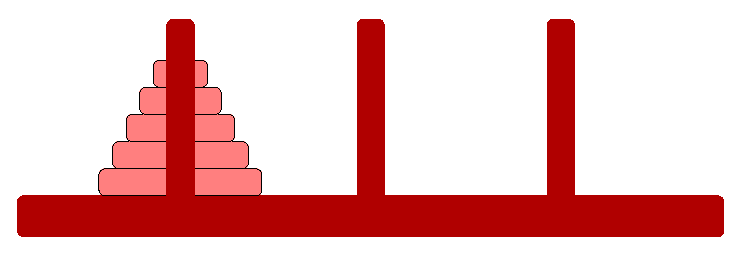
\includegraphics{hanoi.eps}}\\{\sl The Towers of Hanoi}
\end{center}

\section{Variable Scope}
\index{Variables!Scope}
We talk about the ``scope'' of a variable to mean what parts of your
program can see a variable (and change it!) We've seen that subroutines
can see (and change!) all variables we use in the main program, but what
about user defined procedures and functions?

The rules in RTB are somewhat simple, and whilst not identical, are
similar enough to most other progrmaming languages to give you a good
insight.

When a procedure or function is called, the arguments and {\tt LOCAL}
variables store a copy of any variables with the same name, making them
avalable for use inside that procedure or function. When the procedure
ends, then the stored values are copied back into the original variables.

So what happens if a procedure calls another procedure which doesn't
have local variables? Well, the values it sees are those of the last
procedure and not those in the main program. Essentially, RTB propogates
local variables into each new procedure. The easiest way to demonstrate is
by example:
\begin{verbatim}
  100 REM Variable Scope Test
  110 v1 = 123
  120 v2 = 456
  130 PROC test1 (v1)
  140 PRINT "v1 is: "; v1; " v2 is "; v2
  150 END
  300 REM test1
  310 DEF PROC test1 (num1)
  320 LOCAL v1
  330 v1 = 888
  340 PRINT "v1 is: "; v1; " v2 is "; v2; " num1 is: "; num1
  350 PROC test2
  360 ENDPROC
  500 //
  510 REM test2
  520 //
  530 DEF PROC test2
  340 PRINT "v1 is: "; v1; " v2 is "; v2; " num1 is: "; num1
\end{verbatim}

%\addtocontents{toc}{\noindent Foo}
\appendix
\chapter{Colours}\index{Colours}

To keep thing simple, RTB has 16 colours pre-definied for your use. You
can use numbers to represent them, or use the built-in names. The
colours are:

\index{Black}\index{Navy}\index{Green}\index{Teal}\index{Maroon}
\index{Purple}\index{Olive}\index{Silver}\index{Grey}\index{Blue}
\index{Lime}\index{Aqua}\index{Red}\index{Pink}\index{Yellow}\index{White}
\begin{center}
\begin{tabular}{|c|c|c|c|c|c|c|c|c|}
\hline
0 & 1 & 2 & 3 & 4 & 5 & 6 & 7\\
\colorbox{rtb-black}{\hspace{10mm}}&
\colorbox{rtb-navy}{\hspace{10mm}}&
\colorbox{rtb-green}{\hspace{10mm}}&
\colorbox{rtb-teal}{\hspace{10mm}}&
\colorbox{rtb-maroon}{\hspace{10mm}}&
\colorbox{rtb-purple}{\hspace{10mm}}&
\colorbox{rtb-olive}{\hspace{10mm}}&
\colorbox{rtb-silver}{\hspace{10mm}}\\
Black & Navy & Green & Teal & Maroon & Purple & Olive & Silver\\
\hline
\hline
8 & 9 & 10 & 11 & 12 & 13 & 14 & 15\\
\colorbox{rtb-grey}{\hspace{10mm}}&
\colorbox{rtb-blue}{\hspace{10mm}}&
\colorbox{rtb-lime}{\hspace{10mm}}&
\colorbox{rtb-aqua}{\hspace{10mm}}&
\colorbox{rtb-red}{\hspace{10mm}}&
\colorbox{rtb-fuchsia}{\hspace{10mm}}&
\colorbox{rtb-yellow}{\hspace{10mm}}&
\colorbox{rtb-white}{\hspace{10mm}}\\
Grey & Blue & Lime & Aqua & Red & Pink & Yellow & White\\
\hline
\end{tabular}
\end{center}
Note that the colours here are just representative and might not be what
you see on the video screen you are using to run RTB on.

These colours are avalable in both text and graphics modes.

If these 16 colours are not sufficient, then it's possible to use
the full colour pallet of the computer system you are using - this is
usually a 24-bit system with 8 bits for each of Red, Green and Blue,
giving a maximum of 16777216 different colous avalable.

To use the full-colour mode, you need to use the built-in procedure
\begin{itemize}
\item {\tt rgbColour (red, green blue)}
\end{itemize}
where the values of {\tt red, green} and {\tt blue} are numbers from 0
to 255 inclusive.

The extended RGB colours are avalable in graphics modes only. Text is
limited to the standard 16 colours.

\section{A Text Colour Demo}
\index{Text Screen!colour Demo}
There should be a program supplied with your RTB installation called
"colours" which will demo the basic colours in text mode. {\tt LOAD
colours} should obtain it for you, but if it's not avalable then:
\begin{samepage}
\begin{verbatim}
  100 REM Colour test program
  110 //
  120 DIM c$(15)
  130 FOR i = 0 TO 15 CYCLE 
  140   READ c$(i)
  150 REPEAT 
  160 //
  170 CLS 
  180 VTAB = 4
  190 PRINT "Colour test program"
  200 PRINT "==================="
  210 VTAB = 10
  220 FOR bg = 0 TO 15 CYCLE 
  230   FOR i = 0 TO 1 CYCLE 
  240     BCOLOUR = 0
  250     TCOLOUR = bg
  260     PRINT c$(bg);  
  270     FOR fg = 0 TO 7 CYCLE 
  280       PROC testcolour(fg + i * 8, bg)
  290     REPEAT 
  300     PRINT 
  310   REPEAT 
  320 REPEAT 
  330 TCOLOUR = 15
  340 BCOLOUR = 0
  345 END 
  350 //
  360 // Procedure to print some text in the colours supplied
  370 //
  380 DEF PROC testcolour(f, b)
  390 TCOLOUR = f
  400 BCOLOUR = b
  410 PRINT c$(f);  
  420 ENDPROC 
  900 //
  901 DATA " Black  ", " Navy   ", " Green  ", " Teal   "
  902 DATA " Maroon ", " Purple ", " Olive  ", " Silver "
  903 DATA " Grey   ", " Blue   ", " Lime   ", " Aqua   "
  904 DATA " Red    ", " Pink   ", " Yellow ", " White  "
\end{verbatim}
\end{samepage}

\chapter{Numbering Names and Formats}
When numbers get very big or very small, it starts to become hard to
represent them, so we have developed various way to express them. Then
computers came along and things are now somewhat different and potentially
confusing.

The most common way to represent big or small numbers is to write them
in groups of three digits and the International System of Units (SI,
or Syst\`{e}me international d'unit\'{e}s) has a set of standard names
to represent these, however there is a complication. The SI units use
powers of 10 (so 1,000, 1,000,000 and so on), but computers count in
twos (binary), so we've adopted the same names as the decimal units
for computer sizes. A further complication is that some components
manufacturers use the SI units to represent capacities because people
are used to thinking in computers terms, but then find that the decimal
terms are actually smaller. Disk drive manufacturers are frequently
guilty  of this.

The following table gives the most popular definitions you'll encounter:

%\noindent
\begin{tabular}[t]{|c|c|c|c|c|}
\hline
Name	& Kilo		& Mega		& Giga		& Tera			\\
\hline
Decimal	& 1,000		& 1,000,000	& 1,000,000,000	& 1,000,000,000,000	\\
\hline
	& 10$^3$	& 10$^6$	& 10$^9$	& 10$^{12}$		\\
\hline
\hline
Computer& 1024		& 1,048,576	& 1,073,741,824 & 1,099,511,627,776	\\
\hline
	& 2$^{10}$	& 2$^{20}$	& 2$^{30}$	& 2$^{40}$		\\
\hline
\end{tabular}

\noindent
You may see reference to the term {\sl MiB} in some texts - this stands
for Mebi - as in Mebibyte and it used to represent the binary forms. So
2MB is 2,000,000 bytes, but 2MiB is 2,097,152 bytes.

For the most part you can treat the decimal and binary forms as more or
less the same. The MiB format isn't that common yet, but seems to be gaining
popularity in some circles.

\chapter{File Handling functions}
\index{File Handling}

RTB supports reading and writing of files stored on local non-volatile
media (typically disk drives). There are two main methods of file
accessing; sequential and random-access. When you open a file, it is
assigned a numerical {\em ``handle''} and you need to use this handle when
performing other operations on the file. RTB allows you to open multiple
files at the same time, up to a limit set by the implementation. (Usually
8). Each open file will have a unique handle, so you must keep track of
them when manipulating files.

All data written to, or read from a file is textual in nature. You can not
write binary data in RTB. Numbers are stored as literal strings as if they
have been printed on the screen. (And in particular, the format set by
the {\tt NUMFORMAT} instruction is used when printing numbers into files).

\section{Sequential Access}
\index{File Handling!Sequential}
Sequential file access is straightforward. You open a file, then read from
it, or write to it. You can reset the file pointer to the start of the
file using the {\tt REWIND} instruction, so you can write data to a file,
then {\tt REWIND}, then read the data back again. There is no structure
to the file other than what you write into it yourself. ie. if you want
to read the 15th line in a file, then you need to read the preceding 14
lines unless you know the exact line length of each line, then you can use
the {\tt SEEK} instruction to jump to that line, but if the lines are all
different length, then you need to read the while file from start to end,

\section{Random Access}
\index{File Handling!Random}
Random file access is similar to sequential, however it additionally
allows you to split your file into fixed-size records, then
you can {\tt SEEK} to any of these records at random.

There are no special instructions that make a file any different when in
sequential mode to random mode other than those you code yourself. You
must plan the record size (in bytes or characters) before hand and you
must always seek to the correct record in your file before reading or
writing. Each record is then treated like a small sequential file and you
can read and write into it - however you must make sure that you don't
write more data into the record than you have planned for, otherwise
that data will overflow into the next record with unpredictable results.

Random access files can be wasteful of disk space, but they can also
be a fast an versatile method of storing and retrieving data. Most modern
databases use this technique to store data for fast retrieval.

\section{RTB Instructions and functions}

\subsection*{OPEN (filename\$)}
\index{File Handling!OPEN}
The {\tt OPEN} function opens a file and makes it available for reading
or writing and returns the numeric handle assiciated with the file. The
file is created if it doesn't exist, or if it does exist the file pointer
is positioned at the start of the file. To append data to the end of the
file, you need to use the {\tt FFWD} instruction after opening the file.

\subsection*{CLOSE (handle)}
\index{File Handling!CLOSE}
The {\tt CLOSE} instruction closes a file after use and makes sure all
data is securely written to the storage medium.

\subsection*{EOF (handle)}
\index{File Handling!EOF}
The {\tt EOF} function returns a {\tt TRUE} or {\tt FALSE} indication
of the state of the file pointer when reading the file. It is an error
to try to read past the end of the file, so if you are reading a file
with unknown data in it, then you must check at well defined intervals
(e.g. before each {\tt INPUT\#}.

\subsection*{REWIND (handle)\\FFWD (handle)}
\index{File Handling!REWIND}\index{File Handling!FFWD}
Theese instructions move the file pointer back to the start of the file
or to the end of the file respectively. If you want to append data to
the end of an existing file, then you need to call {\tt FFWD} before
writing the data.

\subsection*{SEEK (handle, offset)}
\index{File Handling!SEEK}
The {\tt SEEK} instruction moves the file pointer to any place in the
file. It can even move the file pointer beyond the end of the file in
which case the file is extended. The argument suppled to {\tt SEEK}
is an absolute number of bytes from the start of the file. If you are
using random access files and want to access the 7th record in the file,
then you need to multiple your record size by 7 to get the final location
to seek to.

\subsection*{PRINT\# handle, \dots}
\index{File Handling!PRINT\#}
The {\tt PRINT\#} instruction acts just like the regular {\tt PRINT}
instruction except that it sends data to the file identified by the
supplied file-handle rather than to the screen. Numbers are formatted
according to the settings of {\tt NUMFORMAT}. It is strongly recommended
to only print one item per line if you are going to read those items
back into an RTB program again.
\begin{verbatim}
  100 myFile = OPEN ("testfile.dat")
  110 FFWD (myFile)
  120 PRINT# myFile, "Appended line"
  130 CLOSE (myFile)
\end{verbatim}

\subsection*{INPUT\# handle, variable}
\index{File Handling!INPUT\#}
This works similarly to the regular {\tt INPUT} instruction, but reads
from the file identified by the supplied file-handle rather than from the
keyboard. Note that unlike the regular keyboard {\tt INPUT} instruction,
{\tt INPUT\#} can only read {\em one} variable at a time.
\begin{verbatim}
  100 myFile = OPEN ("testfile.dat")
  110 WHILE NOT EOF (myFile)
  120   INPUT# myFile, line$
  130    PRINT line$
  140 CLOSE (myFile)
\end{verbatim}

\chapter{Serial Port Programming}
\index{Serial Ports}
RTB supports a few instructions to allow you to send and receive data
over serial ports. These go by various names, a common one being RS232.

Moderns PCs often lack a directly connected serial port, so you may have
to use a USB connected device. Using them is the same whether directly
connected or via USB. The important thing to know is the name of the
serial device. For directly connected devices, this might be something
like "/dev/ttyS1", or for USB devices it might be something like
"/dev/ttyUSB0". Occasionally you have find a "/dev/ttyACM0" for some
older USB devices.

\section{SOPEN}
\index{Serial Ports!SOPEN}
This opens a serial device and makes it available for our use. It
takes the name of the serial port and the speed as an argument and
returns a number (the {\em handle}) of the device. We can use this
handle to reference the device and allow us to open several devices at
once. Example:
\begin{verbatim}
  100 arduino = SOPEN ("/dev/ttyUSB0", 115200)
\end{verbatim}
The following baud rates are recognised: {\tt 50, 75, 110, 134, 150,200,
300, 600, 1200, 1800, 2400, 19200, 38400 57600, 115200 and 230400},
but do check your local PC and devices capabilities. The device is
always opened with the data format set to 8 data bits, 1 stop bit and
no parity. All handshaking is turned off.

\section{SCLOSE}
\index{Serial Ports!SCLOSE}
This closes a serial port and frees up and resources used by it. It's
not strictly necessary to do this when you end your program, but it is
considered good practice.
\begin{verbatim}
  120 SCLOSE (arduino)
\end{verbatim}

\section{SGET, SGET\$}
\index{Serial Ports!SGET}\index{Serial Ports!SGET\$}
Fetch a single byte of data from an open serial port and return the
data as either a number or a single-character string. This function will
pause program execution for up to 5 seconds if no data is available. If
there is still not data after 5 seconds, the function will return -1 or
an empty string.
\begin{verbatim}
  130 d = SGET (arduino)
  140 key$ = SGET$ (arduino)
\end{verbatim}

\section{SPUT, SPUT\$}
\index{Serial Ports!SPUT}\index{Serial Ports!SPUT\$}
Send a single byte of data, or a string of characters to an open serial port.
\begin{verbatim}
  130 SPUT (arduino, byte)
  140 SPUT$ (arduino, "Hello")
\end{verbatim}

\section{SREADY}
\index{Serial Ports!SREADY}
Returns the number of characters avalable to be read from an open serial
port. This can be used to poll the device to avoid stalling your program
when there is no data avlable to be read.
\begin{verbatim}
  210 IF SREADY (arduino) THEN PROC getSerialData
\end{verbatim}

\chapter{Raspberry Pi - GPIO Programming}
\index{Raspberry Pi}
RTB supports the on-board GPIO hardware in the Raspberry Pi computer.

\section{PinMode}
\index{Raspberry Pi!PinMode}
This configures the mode of a pin on the Pi's GPIO. It takes
an argument which specifies the mode of the pin - input, output or PWM
output. 
\begin{verbatim}
  220 PinMode (4, 0)
\end{verbatim}
In this example, we're setting pin 4 to be used for input. The modes are;
\begin{description}
\item[0] Input
\item[1] Output
\item[2] PWM Output
\end{description}

\section{DigitalRead}
\index{Raspberry Pi!DigitalRead}
This function allows you to read the state of a digital pin on the
Raspberry Pi. You may need to set the pin mode beforehand to make
sure it's
configured as an input device. It will return {\tt TRUE} or {\tt FALSE}
to indicate an input being high or low respectively.
\begin{verbatim}
  200 PinMode (12, 0) // Set pin 12 to input
  210 if DigitalRead (12) THEN PROC ButtonPushed
\end{verbatim}

\section{DigitalWrite}
\index{Raspberry Pi!DigitalWrite}
This procedure sets a digital pin to the supplied value - 0 for off or
1 for on. As with {\tt DigitalRead}, you may need to set the pin mode
(to output) beforehand.
\begin{verbatim}
  310 PinMode (2, 1) // Set pin 2 to output mode
  320 DigitalWrite (2, 1) // Set output High (on)
  330 Wait (1)
  330 DigitalWrite (2, 0) // Set output Low (off)
\end{verbatim} 

\section{PwmWrite}
\index{Raspberry Pi!PwmWrite}
This procedure outputs a PWM waveform on the selected pin. The pin must
be configured for PWM mode beforehand.
The value set should be between 0 and 1024.
\begin{verbatim}
  310 PinMode (1, 2) // Set pin 1 to PWM output mode
  320 PwmWrite (11, 200)
\end{verbatim} 

\chapter{DRC - Drogon Remote Control Programming}
\index{DRC}
RTB supports the Drogon Remote Control protocol which is used to connect
to devices which interpret the DRC protocol. DRC is typically used with
small micro-controllers such as the Arduino and it allows the control of
the digital and analogue input/output pins to be brought to RTB.

\section{DrcOpen}
\index{DRC!DrcOpen}
This opens a connection to a DRC compatible device and makes it
available for our use. It takes the name of the device as an argument
and returns a number (the {\em handle}) of the device. We can use this
handle to reference the device and allow us to open several devices at
once. Some implementations may have IO devices with fixed named. Example:
\begin{verbatim}
  100 arduino = DrcOpen ("/dev/ttyUSB0")
  110 gpio = DrcOpen ("RPI")
\end{verbatim}
On the Raspberry Pi, you may use the string: {\tt "RPI"}, {\tt RPI-GPIO}
or {\tt RPI-SYS} as the device to open and this will open the on-board
GPIO pins in native wiringPi, GPIO or Sys modes.

\section{DrcClose}
\index{DRC!DrcClose}
This closes a connection to a DRC device and frees up and resources used
by it. It's not strictly necessary to do this when you end your program,
but it is considered good practice.
\begin{verbatim}
  120 DrcClose (arduino)
\end{verbatim}

\section{DrcPinMode}
\index{DRC!DrcPinMode}
This configures the mode of a pin on the remote DRC device. It takes
an argument which specifies the mode of the pin - input, output or PWM
output. Other modes may be available, depending on the device and its 
capabilities. Note that not all devices support all functions.
\begin{verbatim}
  220 DrcPinMode (arduino, 4, 0)
\end{verbatim}
In this example, we're setting pin 4 to be used for input. The modes are;
\begin{description}
\item[0] Input
\item[1] Output
\item[2] PWM Output
\end{description}

\section{DrcDigitalRead}
\index{DRC!DrcDigitalRead}
This function allows you to read the state of a digital pin on the remote
device. You may need to set the pin mode beforehand to make sure it's
configured as an input device. It will return {\tt TRUE} or {\tt FALSE}
to indicate an input being high or low respectively.
\begin{verbatim}
  200 DrcPinMode (arduino, 12, 0) // Set pin 12 to input
  210 if DrcDigitalRead (arduino, 12) THEN PROC ButtonPushed
\end{verbatim}

\section{DrcDigitalWrite}
\index{DRC!DrcDigitalWrite}
This procedure sets a digital pin to the supplied value - 0 for off or
1 for on. As with {\tt DigitalRead}, you may need to set the pin mode
beforehand.
\begin{verbatim}
  310 DrcPinMode (arduino, 2, 1) // Set pin 2 to output mode
  320 DrcDigitalWrite (arduino, 2, 1) // Set output High (on)
  330 Wait (1)
  330 DrcDigitalWrite (arduino, 2, 0) // Set output Low (off)
\end{verbatim} 

\section{DrcAnalogRead}
\index{DRC!DrcAnalogRead}
This function reads an analog channel and returns the result. The value
returned will depend on the hardware you're connected to - for example
the Arduino will return a number from 0 to 1023 representing an input
voltage between 0 and 5 volts. Other devices may have different ranges.
\begin{verbatim}
  250 voltage = DrcAnalogRead (arduino, 4) / 1023 * 5  // Get voltage on pin 4
\end{verbatim}

\section{DrcPwmWrite}
\index{DRC!DrcPwmWrite}
This procedure outputs a PWM waveform on the selected pin. The pin must
be configured for PWM mode beforehand, and depending on the device you
are using, then not all pins on a device may support PWM mode. The value
set should be between 0 and 255.
\begin{verbatim}
  310 DrcPinMode (arduino, 11, 2) // Set pin 11 to PWM output mode
  320 DrcPwmWrite (arduino, 11, 200)
\end{verbatim} 


\backmatter

\begin{theindex}

  \item ABS, 38
  \item Acknowledgements, ii
  \item ACOS, 38
  \item Apple, i, 3
  \item Aqua, 50
  \item Arguments, 37
  \item ASC, 39
  \item ASIN, 38
  \item ATAN, 38
  \item Audience, 1

  \indexspace

  \item BASIC, 5
  \item BBC, i
  \item BCOLOR, 24
  \item BCOLOUR, 24
  \item Black, 50
  \item Blue, 50

  \indexspace

  \item Calculator, 4
  \item CHR\$, 40
  \item CIRCLE, 42
  \item CLEAR, 10
  \item CLOCK, 37
  \item CLS, 37
  \item COLOR, 25
  \item COLOUR, 24, 41
  \item Colours, 50
  \item Command line, 7
    \subitem Edit program lines, 8
    \subitem Editing, 7
    \subitem History, 8
  \item Comments, 11
  \item Commodore PET, i
  \item Conditionals, 29
    \subitem If\dots Then, 26
  \item Constants
    \subitem Built-in, 23
    \subitem Colours, 24
    \subitem Keyboard Keys, 24
  \item CONT, 10
  \item Conventions, 1
  \item Copying, ii
  \item COS, 38

  \indexspace

  \item DATA, 20
  \item DATE\$, 23
  \item DEG, 37
  \item DelSprite, 44
  \item DIM, 16
  \item DIR, 9
  \item DRC, 60
    \subitem DrcAnalogRead, 62
    \subitem DrcClose, 61
    \subitem DrcDigitalRead, 61
    \subitem DrcDigitalWrite, 61
    \subitem DrcOpen, 60
    \subitem DrcPinMode, 61
    \subitem DrcPwmWrite, 62

  \indexspace

  \item ED, 10
  \item ELLIPSE, 43
  \item END, 37
  \item EXIT, 10
  \item EXP, 38

  \indexspace

  \item FALSE, 24
  \item File Handling, 53
    \subitem CLOSE, 54
    \subitem EOF, 54
    \subitem FFWD, 55
    \subitem INPUT\#, 55
    \subitem OPEN, 54
    \subitem PRINT\#, 55
    \subitem Random, 54
    \subitem REWIND, 55
    \subitem SEEK, 55
    \subitem Sequential, 53
  \item File names, 10
  \item Flow Control, 12
  \item Functions, 37

  \indexspace

  \item GET, 23
  \item GET\$, 23
  \item GHEIGHT, 41
  \item GOSUB, 12
    \subitem Controversy, 13
  \item GOTO, 12
    \subitem Controversy, 13
    \subitem Respect, 13
  \item GR, 42
  \item Graphics, 41
  \item Green, 50
  \item Grey, 50
  \item GWIDTH, 24, 41

  \indexspace

  \item HASH, 39
  \item HEIGHT, 24
  \item HGR, 42
  \item HLINE, 42
  \item HTAB, 24
  \item HVTAB, 37

  \indexspace

  \item IF
    \subitem ELSE, 27
    \subitem ENDIF, 26
    \subitem Multiple Lines, 26
    \subitem THEN, 26
  \item Immediate mode, 4
  \item Immediate mode commands, 9
  \item INKEY, 23
  \item Input, 17
  \item INT, 38

  \indexspace

  \item LEFT, 44
  \item LEFT\$, 40
  \item LEN, 39
  \item LET, 15
  \item Lime, 50
  \item LINE, 42
  \item LINETO, 42
  \item Linux, 3
  \item LIST, 9
  \item LOAD, 9
  \item LoadSprite, 44
  \item LOG, 38
  \item Loops, 32
    \subitem BREAK, 36
    \subitem CONTINUE, 36
    \subitem CYCLE, 32, 34
    \subitem DO, 32, 34
    \subitem FOR, 34
    \subitem NEXT, 35
    \subitem REPEAT, 32
    \subitem STEP, 35
    \subitem UNTIL, 33
    \subitem WHILE, 33

  \indexspace

  \item Mac, 3
  \item Maroon, 50
  \item Matryoshka dolls, 47
  \item MAX, 39
  \item MID\$, 40
  \item MIN, 39
  \item Modes, 4
  \item MOVE, 43
  \item MOVETO, 44

  \indexspace

  \item Navy, 50
  \item NEW, 9
  \item Numbers, 14
  \item Numeric Operators, 15
  \item Numerical Functions, 38
  \item NUMFORMAT, 37

  \indexspace

  \item Olive, 50
  \item ORIGIN, 43
  \item Output, 17

  \indexspace

  \item PC, 3
  \item PENDOWN, 43
  \item PENUP, 43
  \item PI, 23
  \item PI2, 23
  \item Pink, 50
  \item PLOT, 42
  \item PlotSprite, 44
  \item PolyPlot, 43
  \item PolyStart, 43
  \item Precedence, 15
  \item Preface, i
  \item Procedures, 37
  \item Prompt, 3
  \item Purple, 50

  \indexspace

  \item RAD, 37
  \item Raspberry Pi, 3, 58
    \subitem DigitalRead, 58
    \subitem DigitalWrite, 59
    \subitem PinMode, 58
    \subitem PwmWrite, 59
  \item READ, 20
  \item RECT, 43
  \item Recursion, 47
    \subitem Factorial, 47
    \subitem Towers of Hanoi, 48
  \item Red, 50
  \item RENUMBER, 6, 10
  \item RESTORE, 20
  \item rgbColour, 42
  \item RIGHT, 44
  \item RIGHT\$, 40
  \item RND, 38
  \item RUN, 9
  \item Run mode, 4

  \indexspace

  \item SAVE, 9
  \item SAVENN, 9
  \item SaveScreen, 42
  \item Scientific Notation, 14
  \item SEED, 24
  \item Serial Ports, 56
    \subitem SCLOSE, 57
    \subitem SGET, 57
    \subitem SGET\$, 57
    \subitem SOPEN, 56
    \subitem SPUT, 57
    \subitem SPUT\$, 57
    \subitem SREADY, 57
  \item SGN, 38
  \item Silver, 50
  \item SIN, 38
  \item Sinclair, i
  \item SPACE\$, 40
  \item SQRT, 38
  \item STOP, 10, 37
  \item Stored program mode, 5
  \item STR\$, 40
  \item String Functions, 40
  \item Strings, 14
  \item SWAP, 37

  \indexspace

  \item TAN, 38
  \item TANGLE, 24, 41
  \item TCOLOR, 24
  \item TCOLOUR, 24
  \item Teal, 50
  \item Text Screen
    \subitem colour Demo, 51
  \item TIME, 23
  \item TIME\$, 23
  \item Trademarks, ii
  \item TRIANGLE, 43
  \item TROFF, 10
  \item TRON, 10
  \item TRUE, 23
  \item TTHEIGHT, 24
  \item TWIDTH, 24

  \indexspace

  \item UPDATE, 42
  \item User defined Procedures and Functions, 45
    \subitem =, 46
    \subitem DEF, 45
    \subitem DEF PROC, 45
    \subitem Functions, 46
    \subitem PROC, 46
    \subitem Procedures, 45

  \indexspace

  \item VAL, 39
  \item Variables, 14
    \subitem Arrays, 16
    \subitem Assignment, 15
    \subitem Associative Arrays, 16
    \subitem Built-in, 23
    \subitem Map, 16
    \subitem Names, 14
    \subitem Read Only, 23
    \subitem Read/Write, 24
    \subitem Scope, 48
    \subitem Types, 14
  \item VERSION, 10
  \item VLINE, 42
  \item VTAB, 24

  \indexspace

  \item WAIT, 37
  \item Warning, 2
  \item Warranty, ii
  \item White, 50

  \indexspace

  \item Yellow, 50

\end{theindex}


\end{sffamily}
\end{document}
